\documentclass[final]{beamer}
\mode<presentation>
  {
  \usetheme{Rutgers}
  }
  \usepackage{amsmath,amsthm, amssymb, latexsym}
  \boldmath
  \usepackage[english]{babel}
  \usepackage[latin1]{inputenc}
  \usepackage{lmodern}
  \usepackage[orientation=portrait,size=a0,scale=1.4,debug]{beamerposter}
  
\usepackage{myalgorithm}
\usepackage{wrapfig}
\usepackage[noend]{myalgorithmic}
\usepackage{multirow}
\usepackage{multicol}
\usepackage{graphicx,wrapfig,lipsum}
\usepackage[font=footnotesize]{caption}


  %%%%%%%%%%%%%%%%%%%%%%%%%%%%%%%%%%%%%%%%%%%%%%%%%%%%%%%%%%%%%%%%%%%%%%%%%%%%%%%%%
  \title[Dataset]{Object Detection and Pose Estimation for Robotic Manipulation \\ using Physics Simulation and Monte-Carlo Tree Search}
  \author[Mitash]{Chaitanya Mitash, Abdeslam Boularias and Kostas E. Bekris}
  \institute[RutgersFUES]{Department of Computer Science, Rutgers, the State University of New Jersey}
  %%%%%%%%%%%%%%%%%%%%%%%%%%%%%%%%%%%%%%%%%%%%%%%%%%%%%%%%%%%%%%%%%%%%%%%%%%%%%%%%%
  \newlength{\blocklen}
  \begin{document}
  \setlength{\blocklen}{0.49\textwidth}
  \begin{frame}{} 
    \vspace {-0.5in}
    \begin{columns}[t]
	\begin{column}{0.50\textwidth}
		\begin{block}{\large Motivation for autonomous data generation}
		    	\begin{columns}[T]
		    		\centering
		    		\begin{column}{0.60\textwidth}
					    {\bf \quad Motivation:}
					    \begin{itemize}
						    \item State-of-the-art methods use Convolutional Neural Network (CNN) to perform object segmentation.
						    \item CNNs need access to a large set of labeled data, which requires intensive human labor.
						    \item Current techniques for generating synthetic dataset suffers from dataset bias as they lack realism.
					    \end{itemize}
					    \vspace{0.8in}
					    {\bf\quad Objective:}
					    \begin{itemize}
					    \item Generate a physically-realistic labeled dataset in an autonomous manner to train a CNN for object detection.
					    \end{itemize}
					\end{column}
					\begin{column}{0.40\textwidth}
						\centering
						\vspace{-0.2in}
						\begin{figure}[h]
							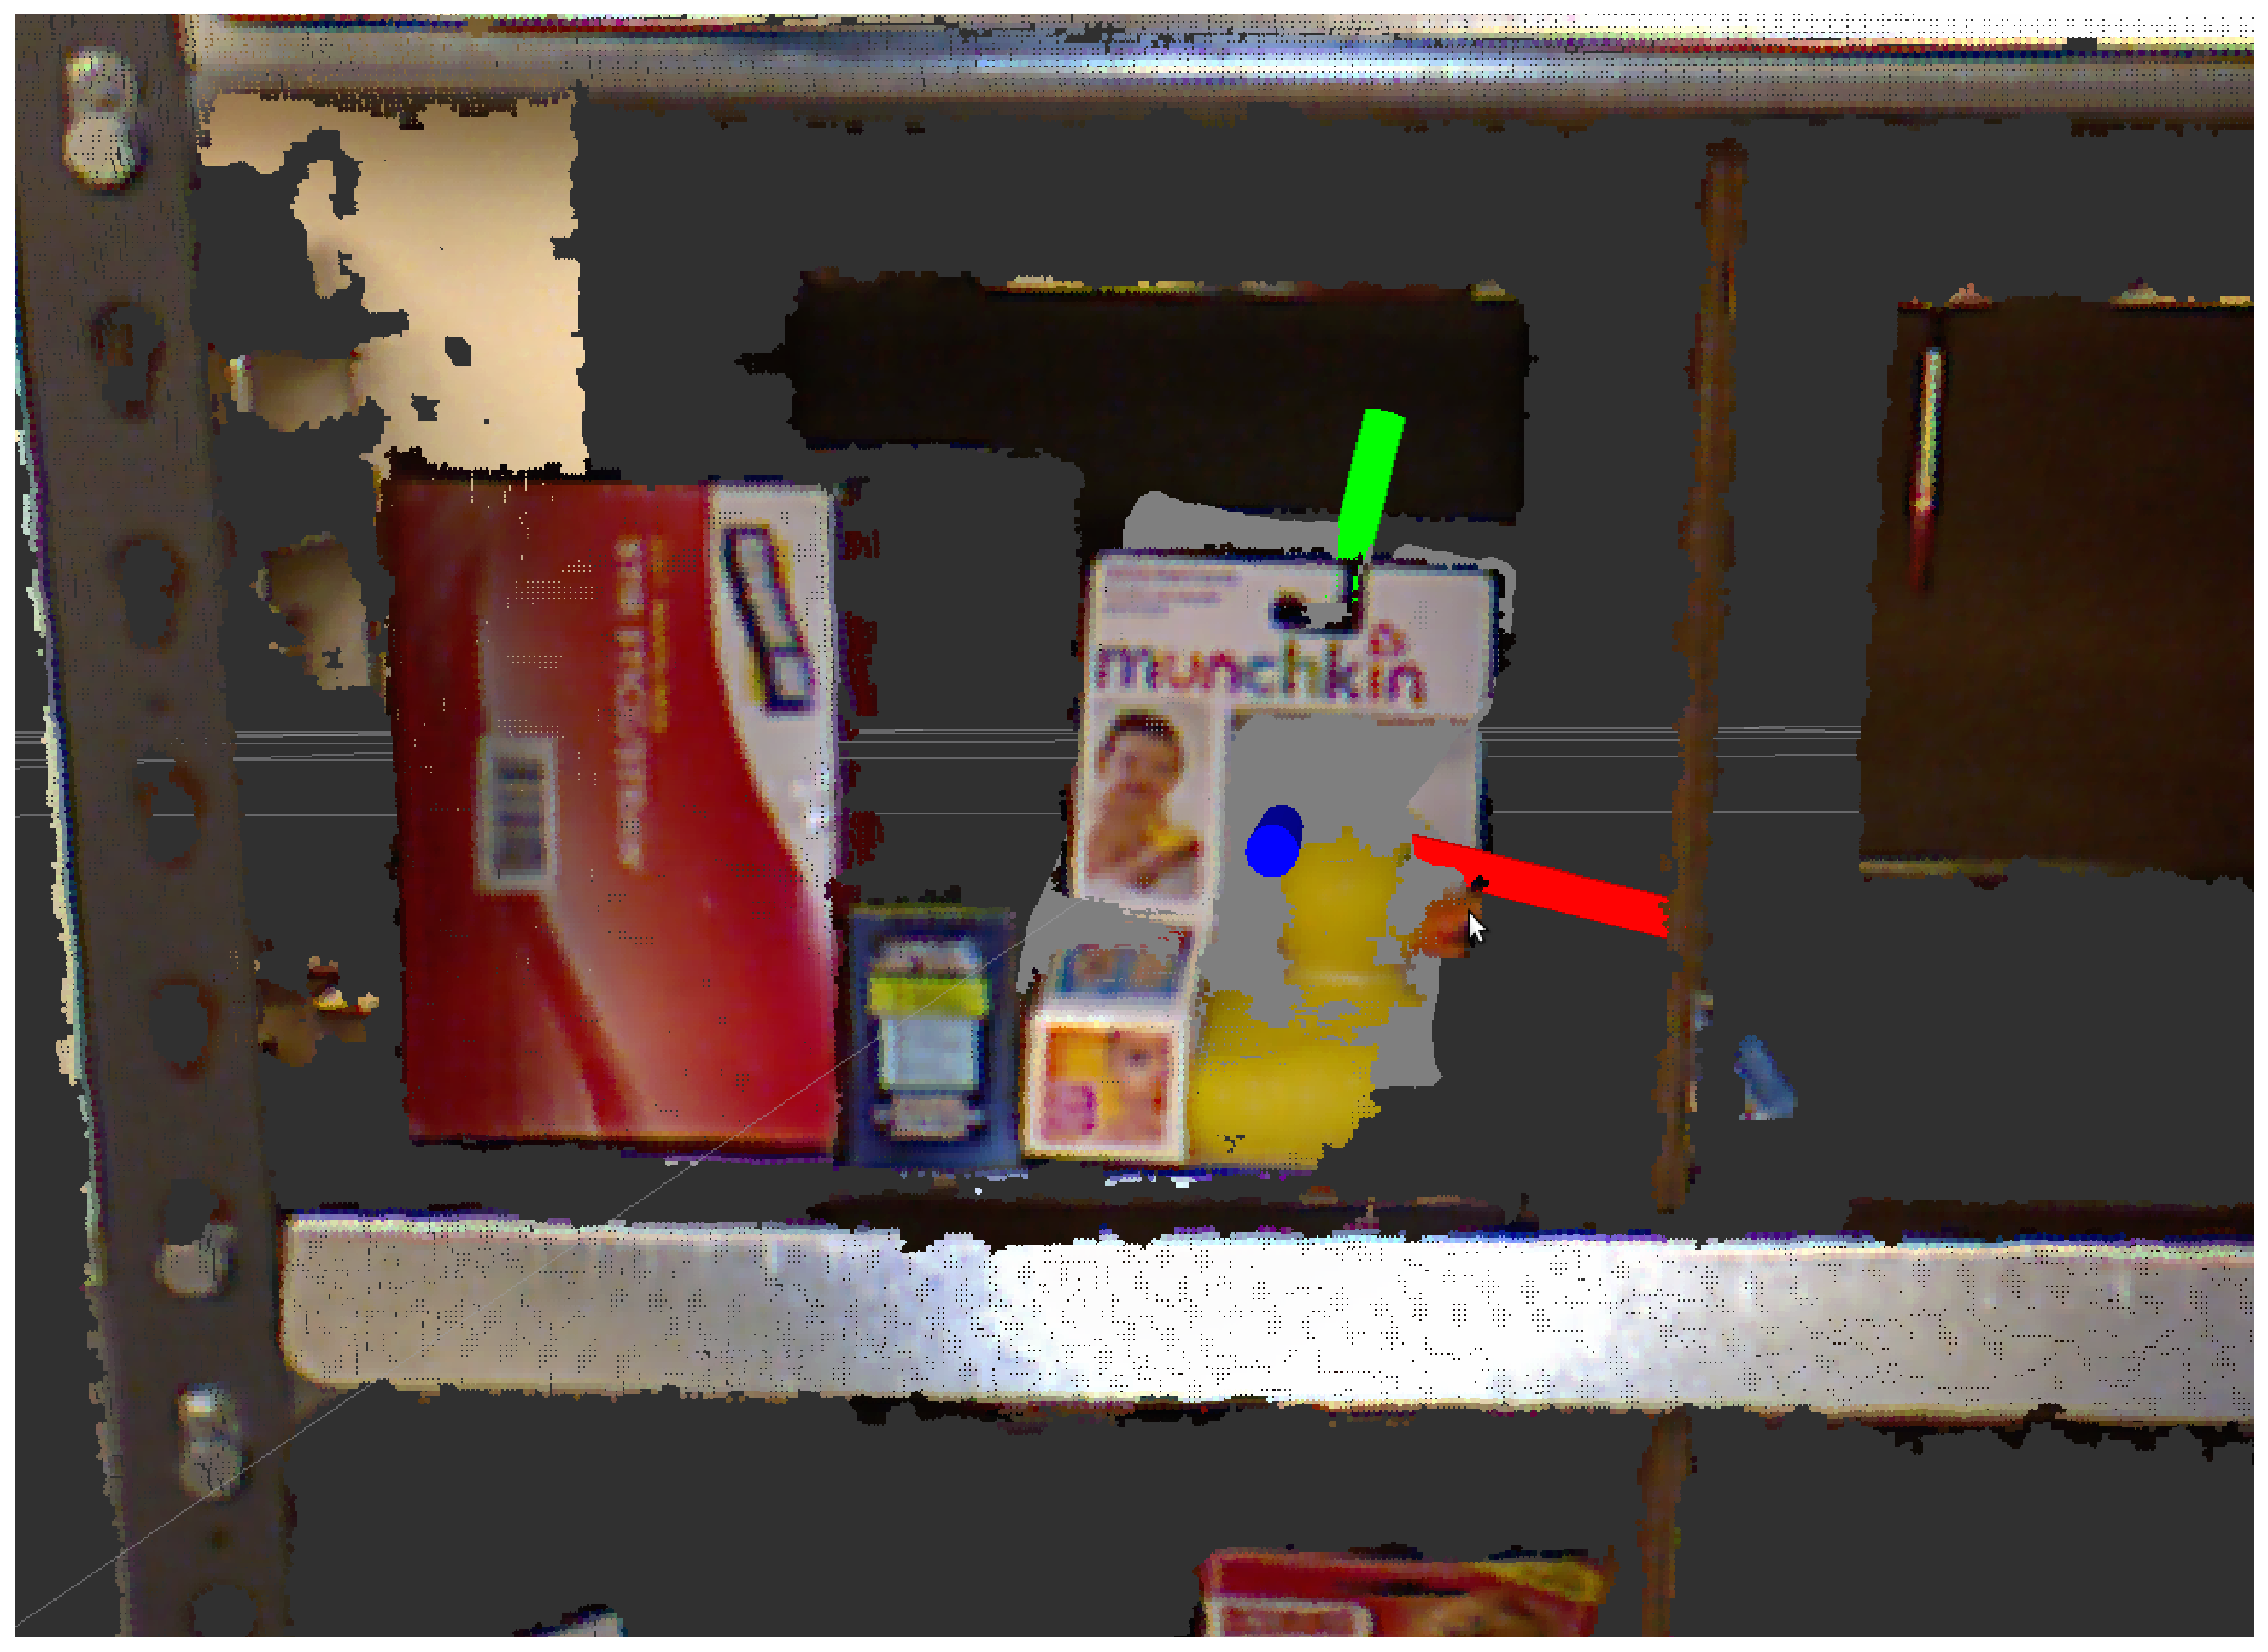
\includegraphics[width=0.75\textwidth]{manual_rutgers}
							\vspace{0.1in}
							\caption{Rutgers RGBD dataset with manual annotation}
						\end{figure}
						\vspace{0.3in}
						\begin{figure}[h]
							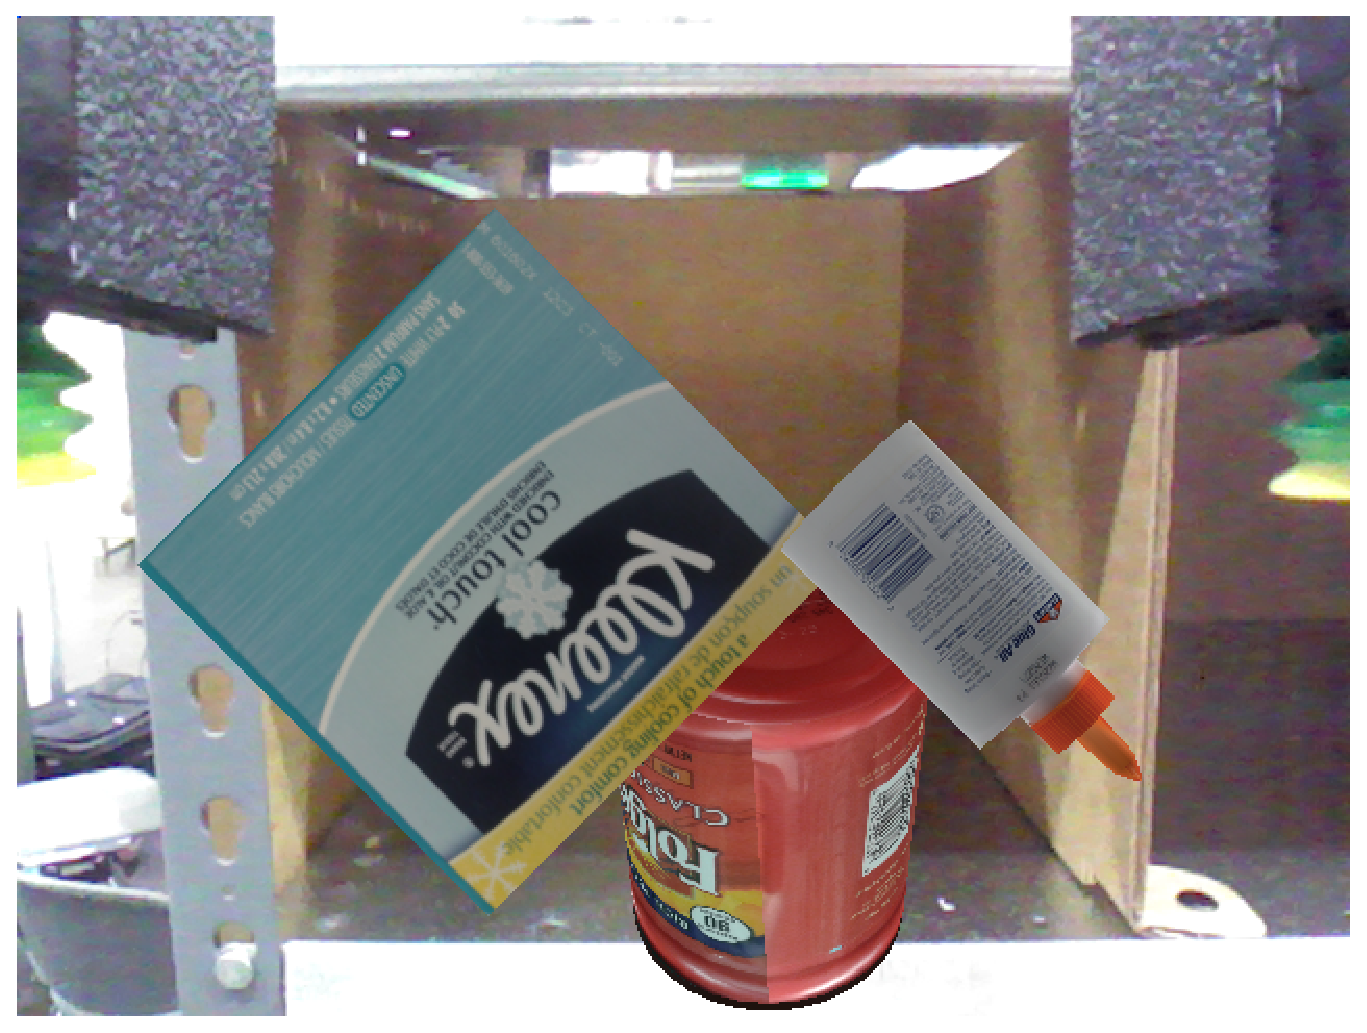
\includegraphics[width=0.75\textwidth]{unreal_syn}
							\vspace{0.1in}
							\caption{Physically unrealistic synthetic dataset generation}
						\end{figure}
					\end{column}
				\end{columns}
		\end{block}
	\end{column}
	\begin{column}{0.50\textwidth}
		\begin{block}{\large Using Physics Simulation to generate training dataset}
		\centering
		    \begin{itemize}
			    \item Environmental and geometric constraints are used to generate datasets for \\setups such as shelf bin and table-top.
			    \item Each scene is generated by randomly sampling object poses from a domain specified for the setup.
			    \item Physics simulation is performed for generating physically realistic scenes so that the training dataset captures appropriate object scales and occlusions.
		    \end{itemize}
		    \vspace{0.2in}
		    \begin{figure}[h]
				\includegraphics[width=0.80\textwidth]{physim}
				\caption{Pipeline for data generation using physics simulation}
			\end{figure}
		\end{block}
	\end{column}
\end{columns}	
		    

    \vfill
    \begin{columns}[t]
	\begin{column} {0.42\textwidth}
		\begin{block}{\large Dataset Generation Tool}
			\centering
			\begin{itemize}
				\item The software tool for dataset generation is publicly released and can be found at \url{https://github.com/cmitash/physim-dataset-generator}
				\item It uses the {\tt Blender} python API for simulation and rendering.
				\item The repository also includes CAD models for 16 objects from {\it Amazon Picking Challenge 2016}.
				\item The camera parameters, choice of environment, and lighting options are provided as tunable parameters.
				\item The tool could be used to generate scenes with either bounding-box or pixel-wise class labels for objects.
			\end{itemize}
			\begin{columns}[t]
			\begin{column} {0.33\textwidth}
			\begin{figure}[h]
				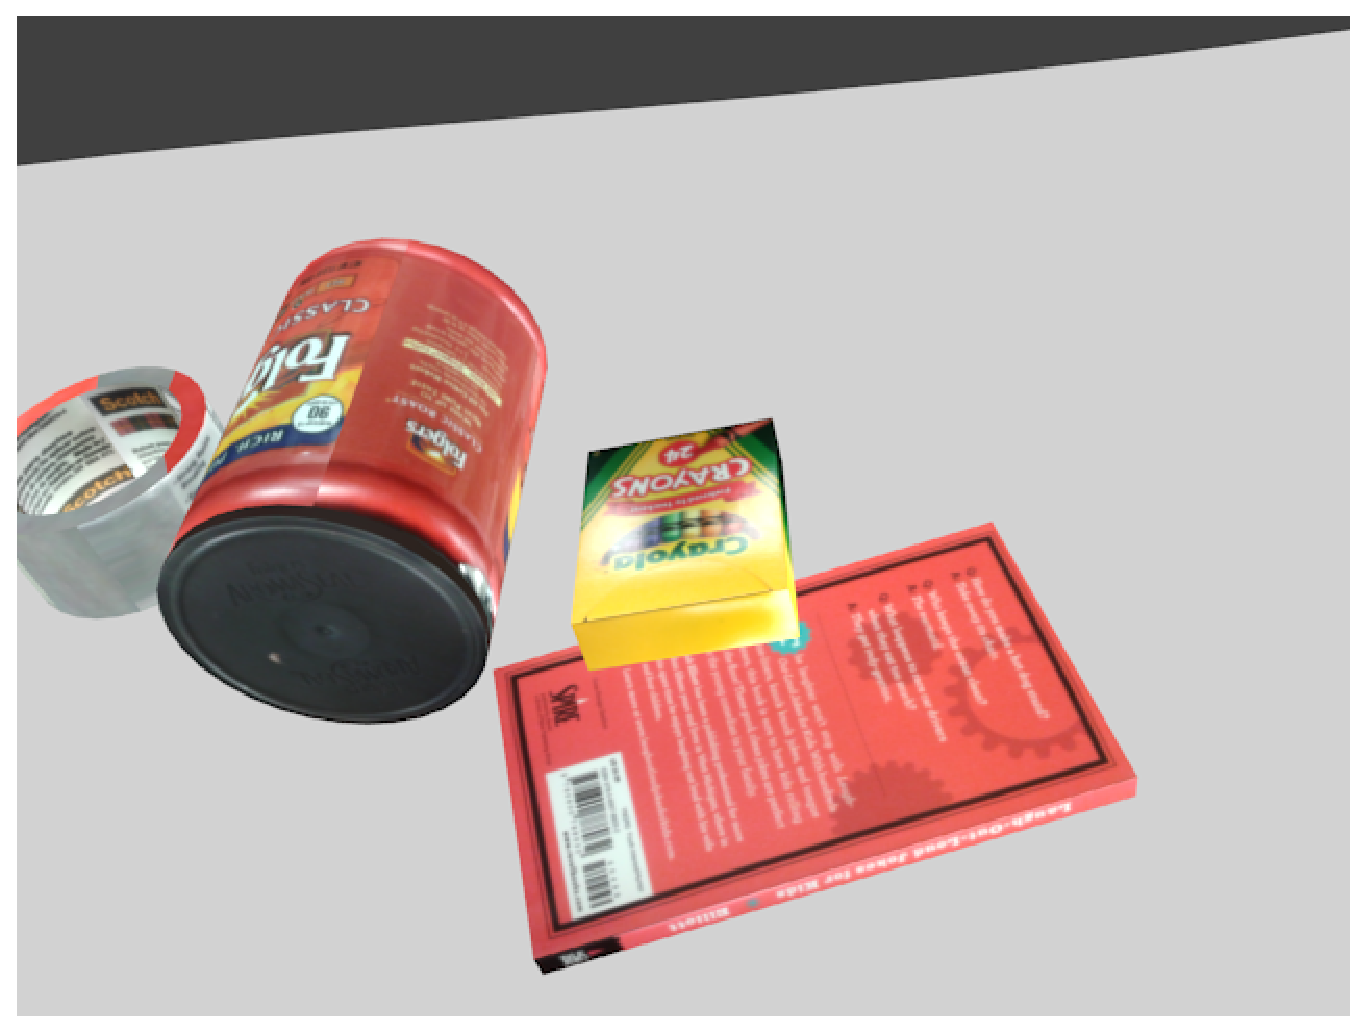
\includegraphics[width=0.8\textwidth]{ex1}
				\caption{example image}
			\end{figure}
			\end{column}
			\begin{column} {0.33\textwidth}
			\begin{figure}[h]
				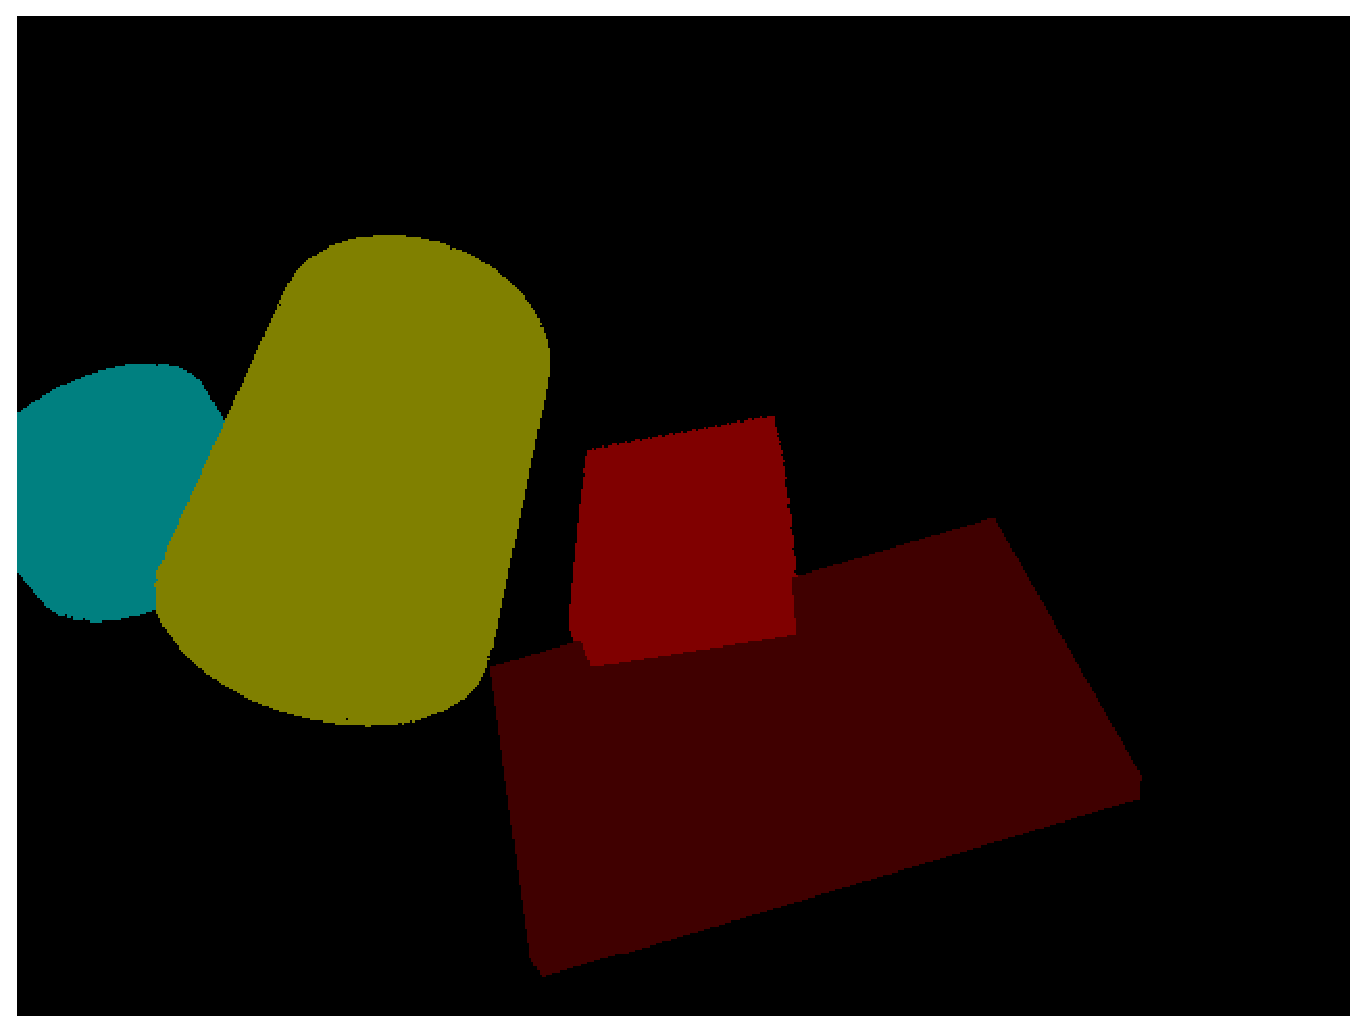
\includegraphics[width=0.8\textwidth]{ex2}
				\caption{pixel-wise labeling}
			\end{figure}
			\end{column}
			\begin{column} {0.33\textwidth}
			\begin{figure}[h]
				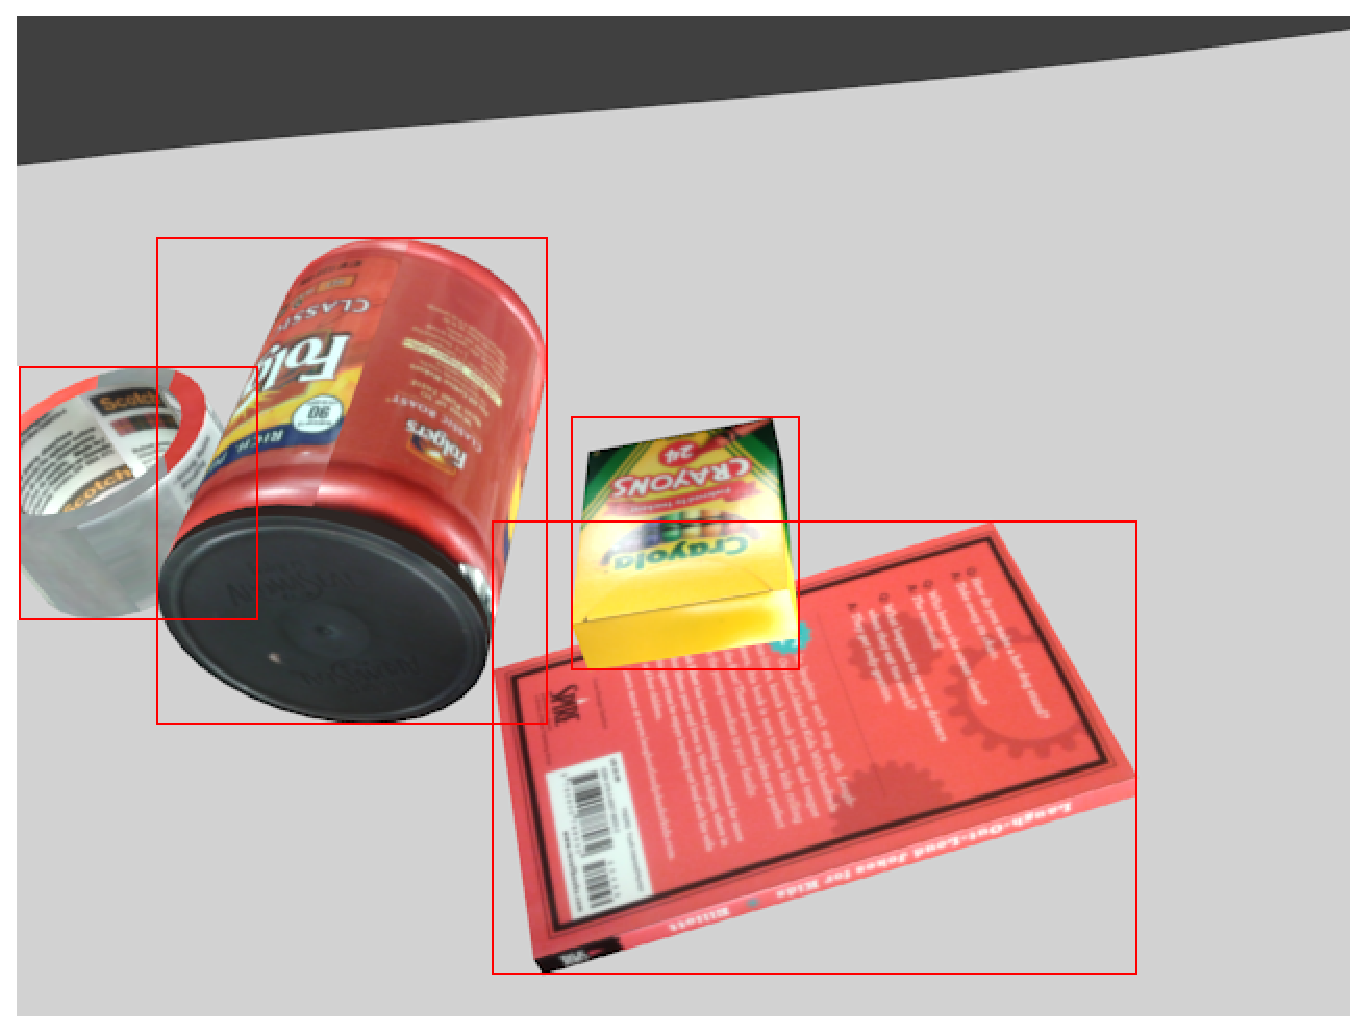
\includegraphics[width=0.8\textwidth]{ex3}
				\caption{bounding-box labeling}
			\end{figure}
			\end{column}
			\end{columns}
		\end{block}
	\end{column}

	\begin{column}{0.30\textwidth}
		\begin{block} {\large Evaluating Object Detection}
			\centering
			\begin{itemize}
				\item Evaluation is performed on {\tt Shelf \& Tote} benchmark dataset.
				 % released by Team MIT-Princeton participating in APC 2016. 
				% Reported result is detection success(\%) i.e Intersection-over-union $>$ 50\%
				\item {\tt Faster-RCNN} is trained using approximately 2000 physically-realistic scenes.The small number helps avoid overfitting with respect to texture and scene illumination.
			\end{itemize}
			\begin{figure}[h]
				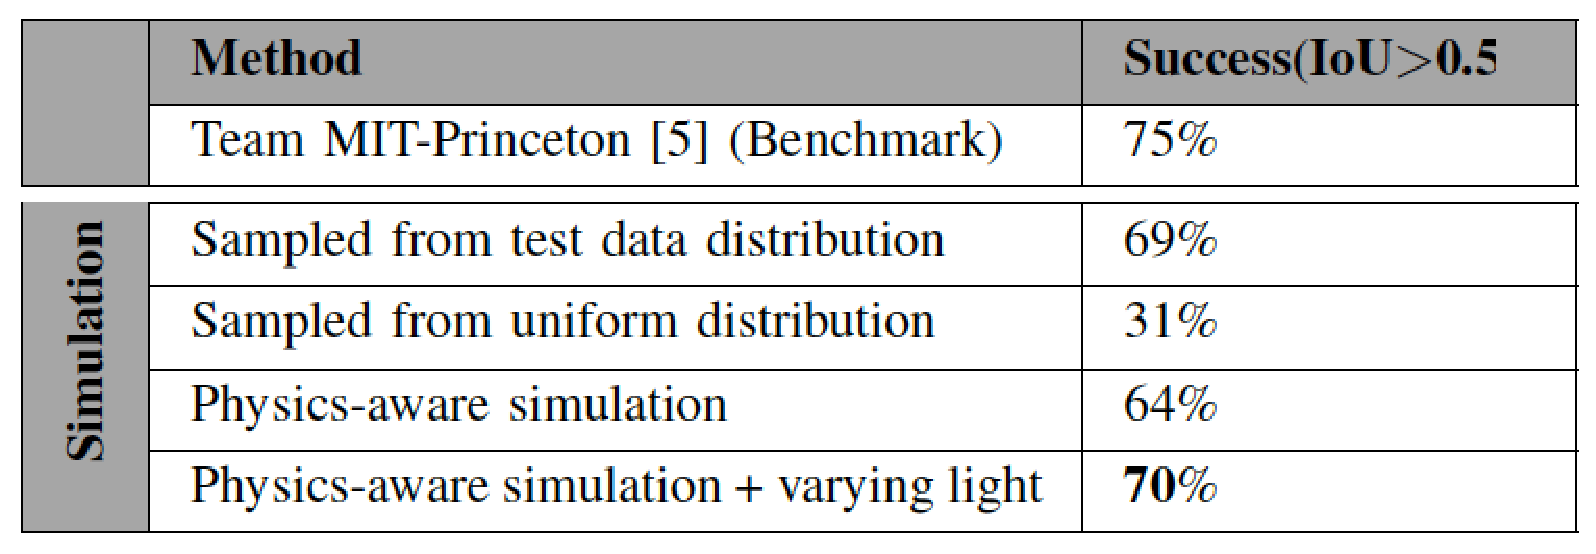
\includegraphics[width=0.9\textwidth]{detectRes}
			\end{figure}
			\vspace{-0.1in}
			\begin{figure}[h]
				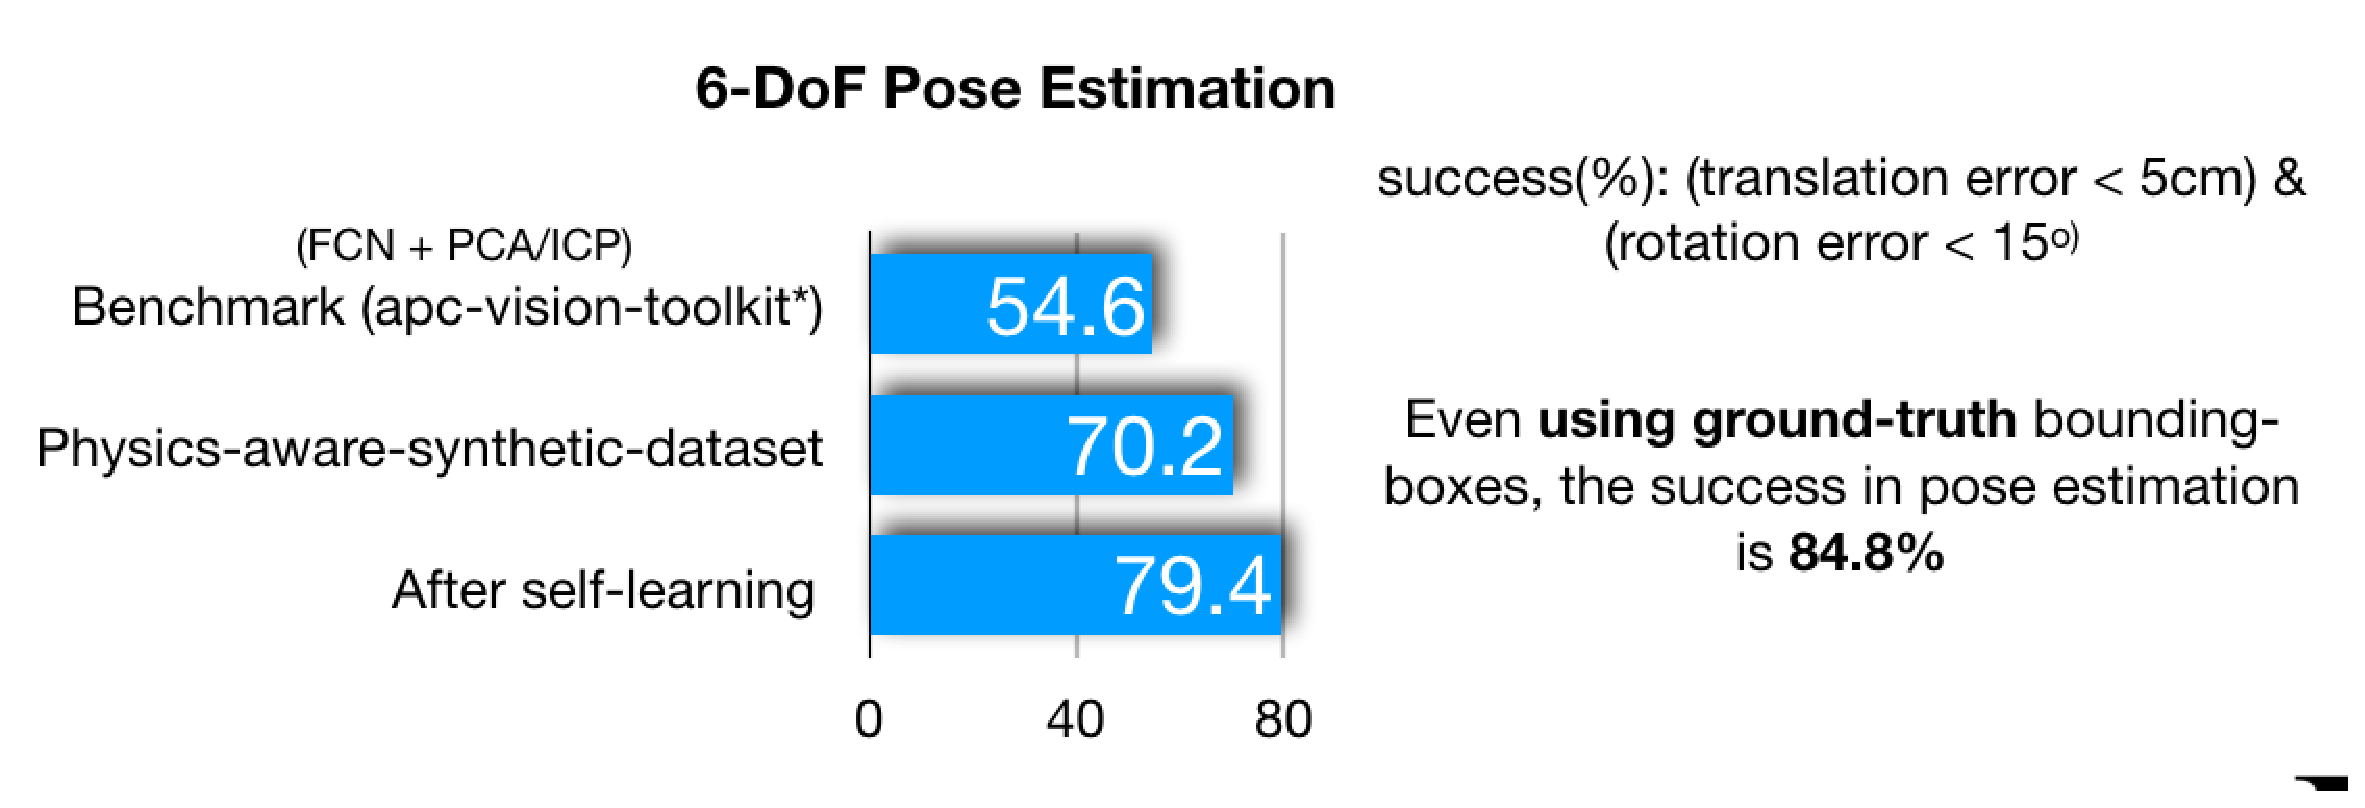
\includegraphics[width=0.9\textwidth]{eval_pose}
			\end{figure}
		\end{block}
	\end{column}
	\begin{column}{0.28\textwidth}
		\begin{block}{\large Motivation for MCTS}
			\centering
			\begin{itemize}
				\item Model-matching to individual object segments often result in pose estimates of objects that are physically inconsistent with other objects.
				\item Efficient search technique is required to search over the combination of individual pose hypotheses which best explains the observed scene.
			\end{itemize}
			\vspace{0.3in}
			\begin{columns}[t]
			\begin{column} {0.45\textwidth}
			\begin{figure}[h]
				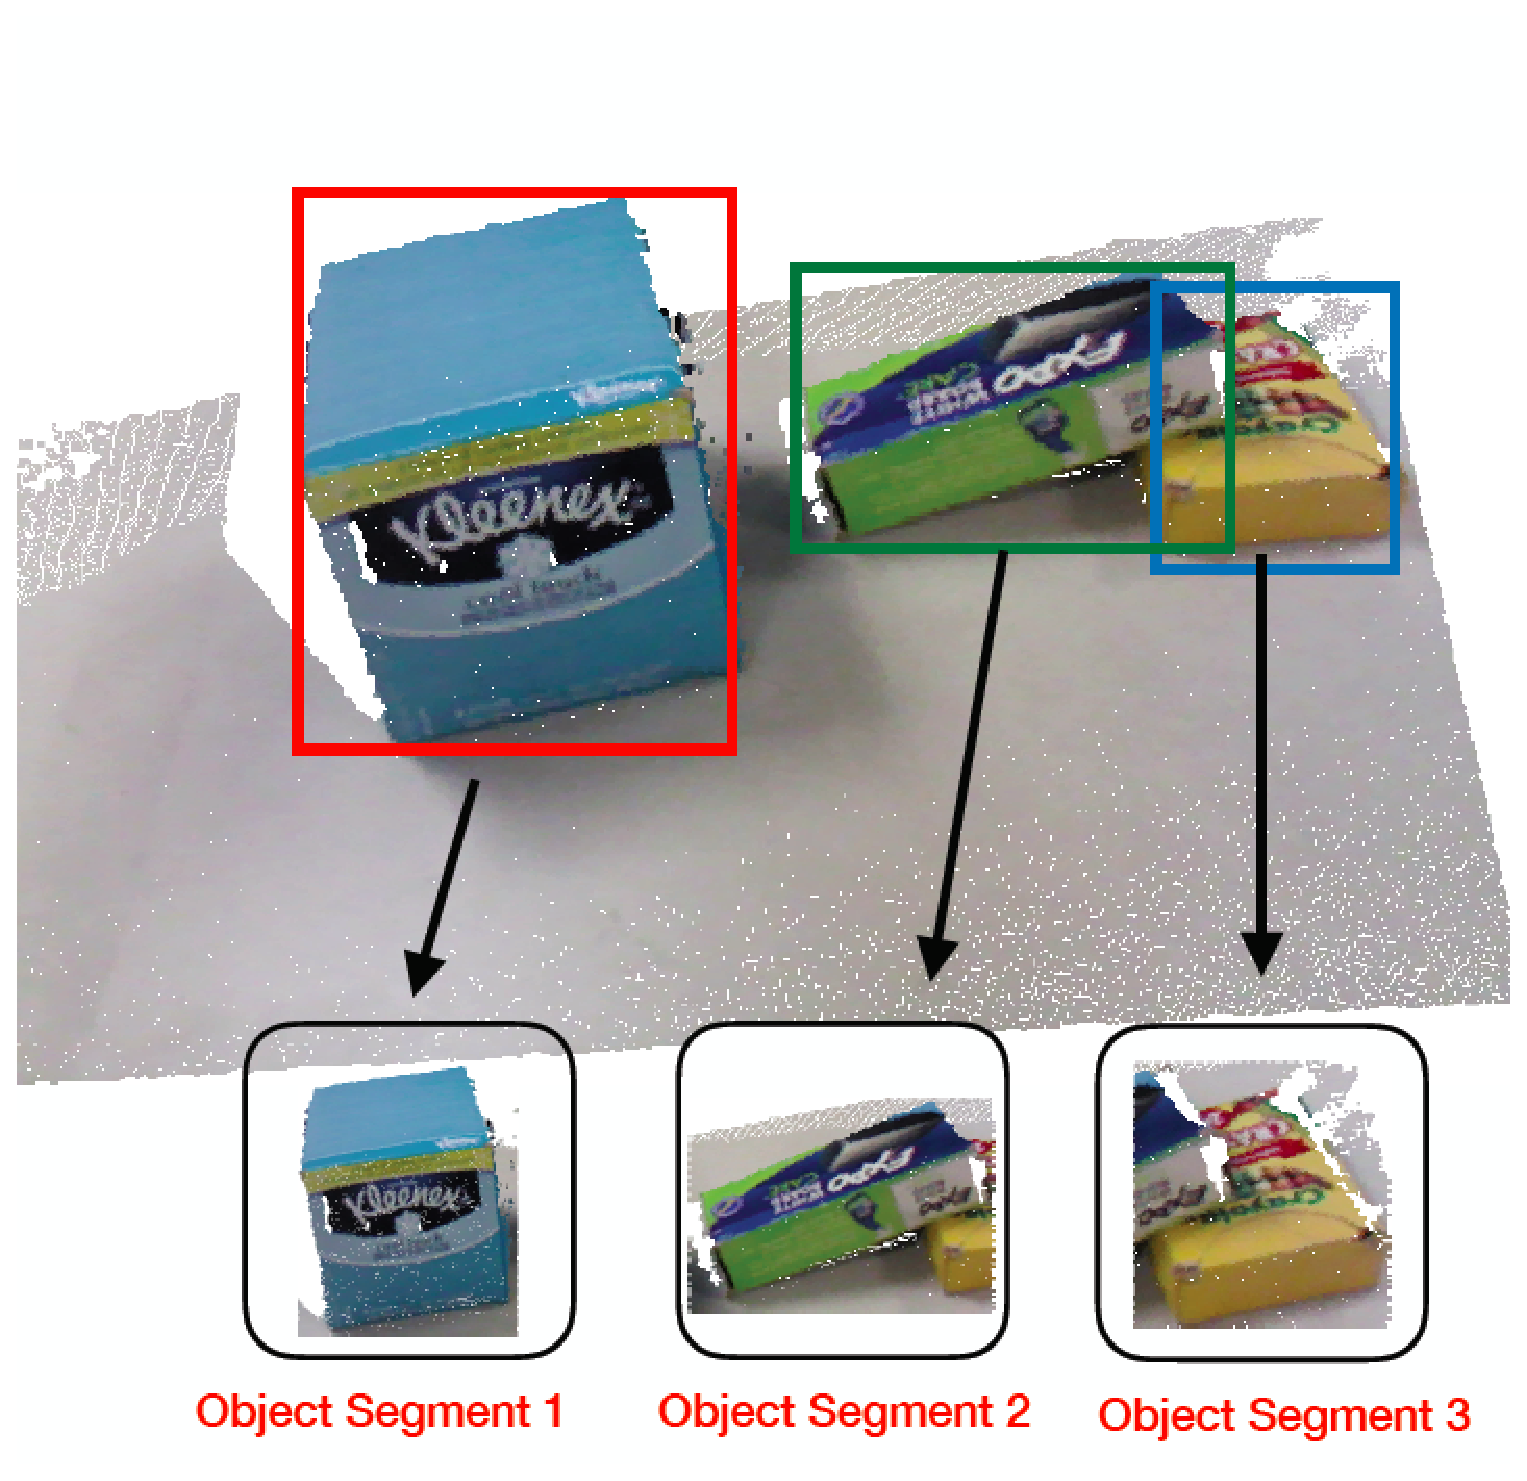
\includegraphics[width=0.75\textwidth]{obj_seg}
				\caption{Object segmentation with Faster-RCNN}
			\end{figure}
			\end{column}
			\begin{column} {0.45\textwidth}
			\begin{figure}[h]
				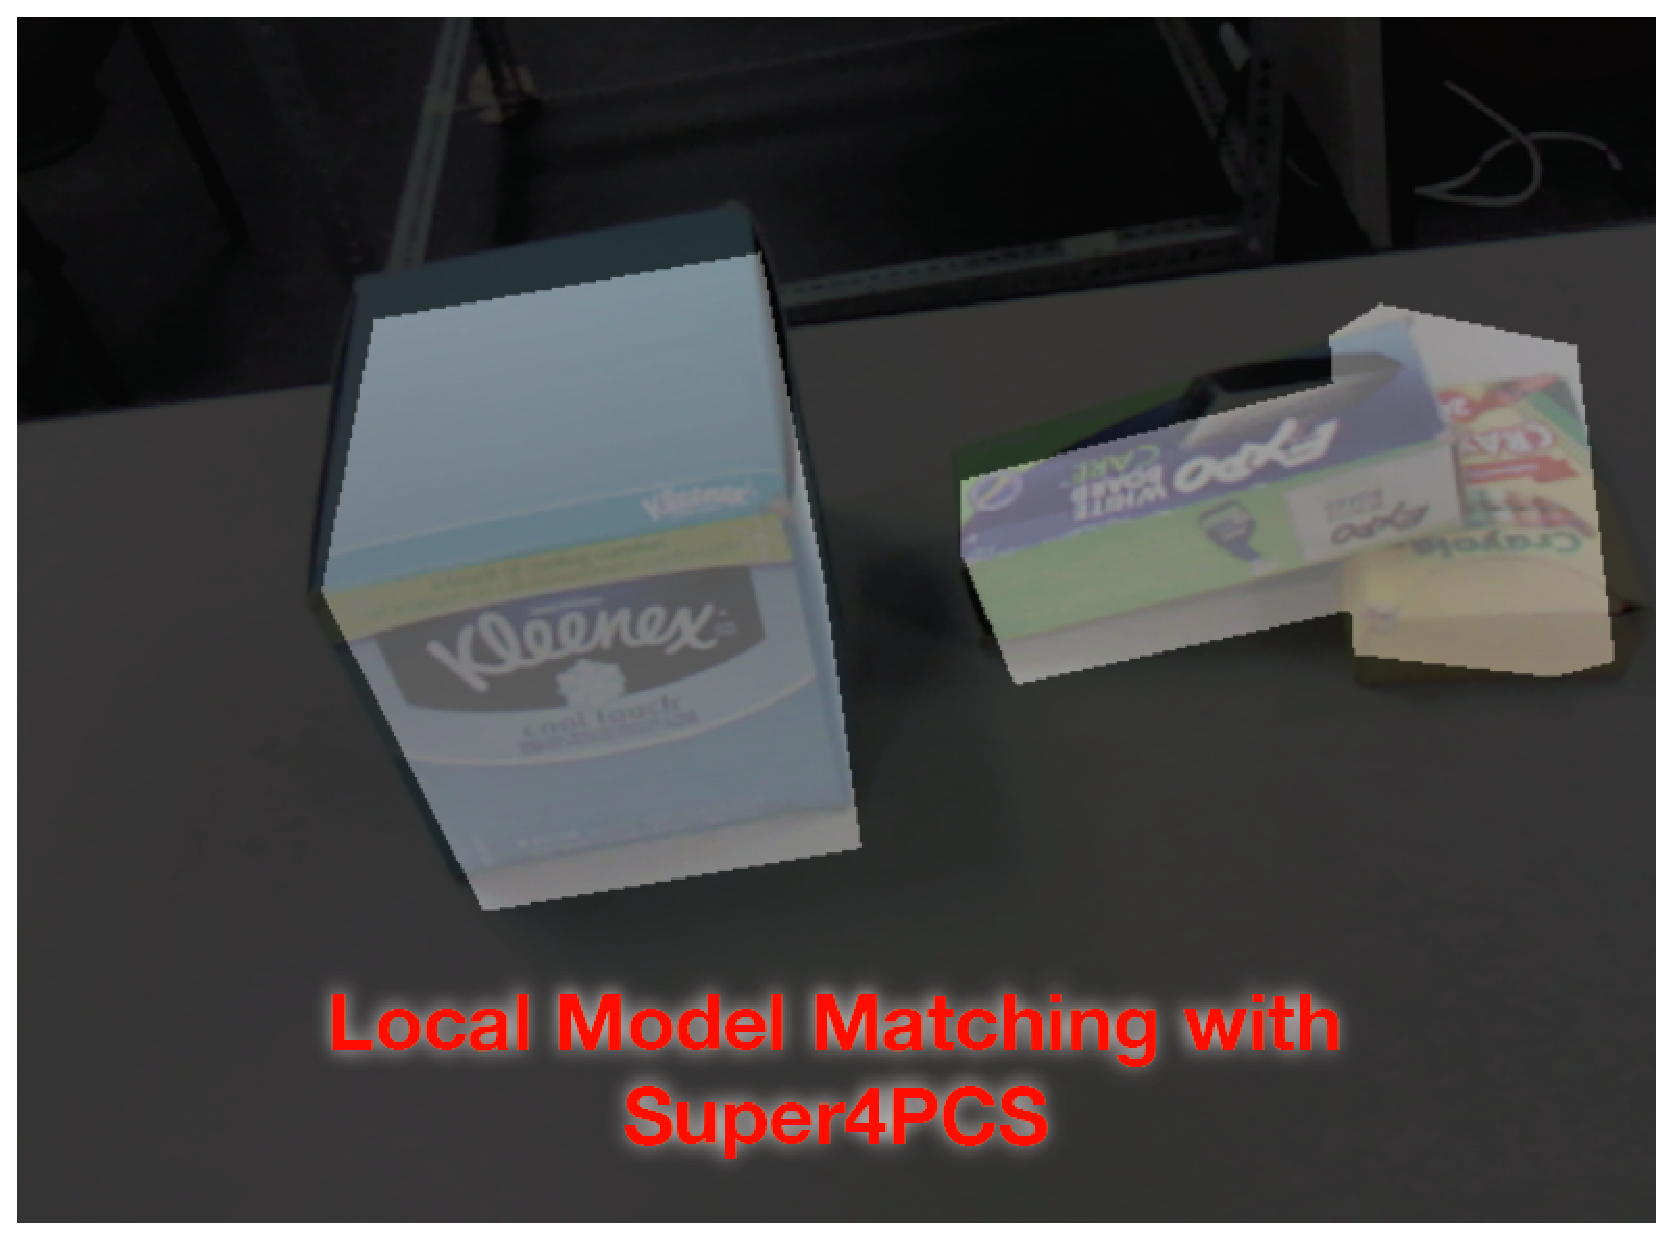
\includegraphics[width=0.9\textwidth]{local_match}
				\caption{Result of model-matching using Super4PCS}
			\end{figure}
			\end{column}
			\end{columns}
		\end{block}
	\end{column}
\end{columns}




    \vfill
    \begin{columns}[t]
	\begin{column}{0.70\textwidth}
		\begin{block}{\large Pose Estimation using Monte Carlo Tree Search}
			\centering
			\begin{figure}[h]
				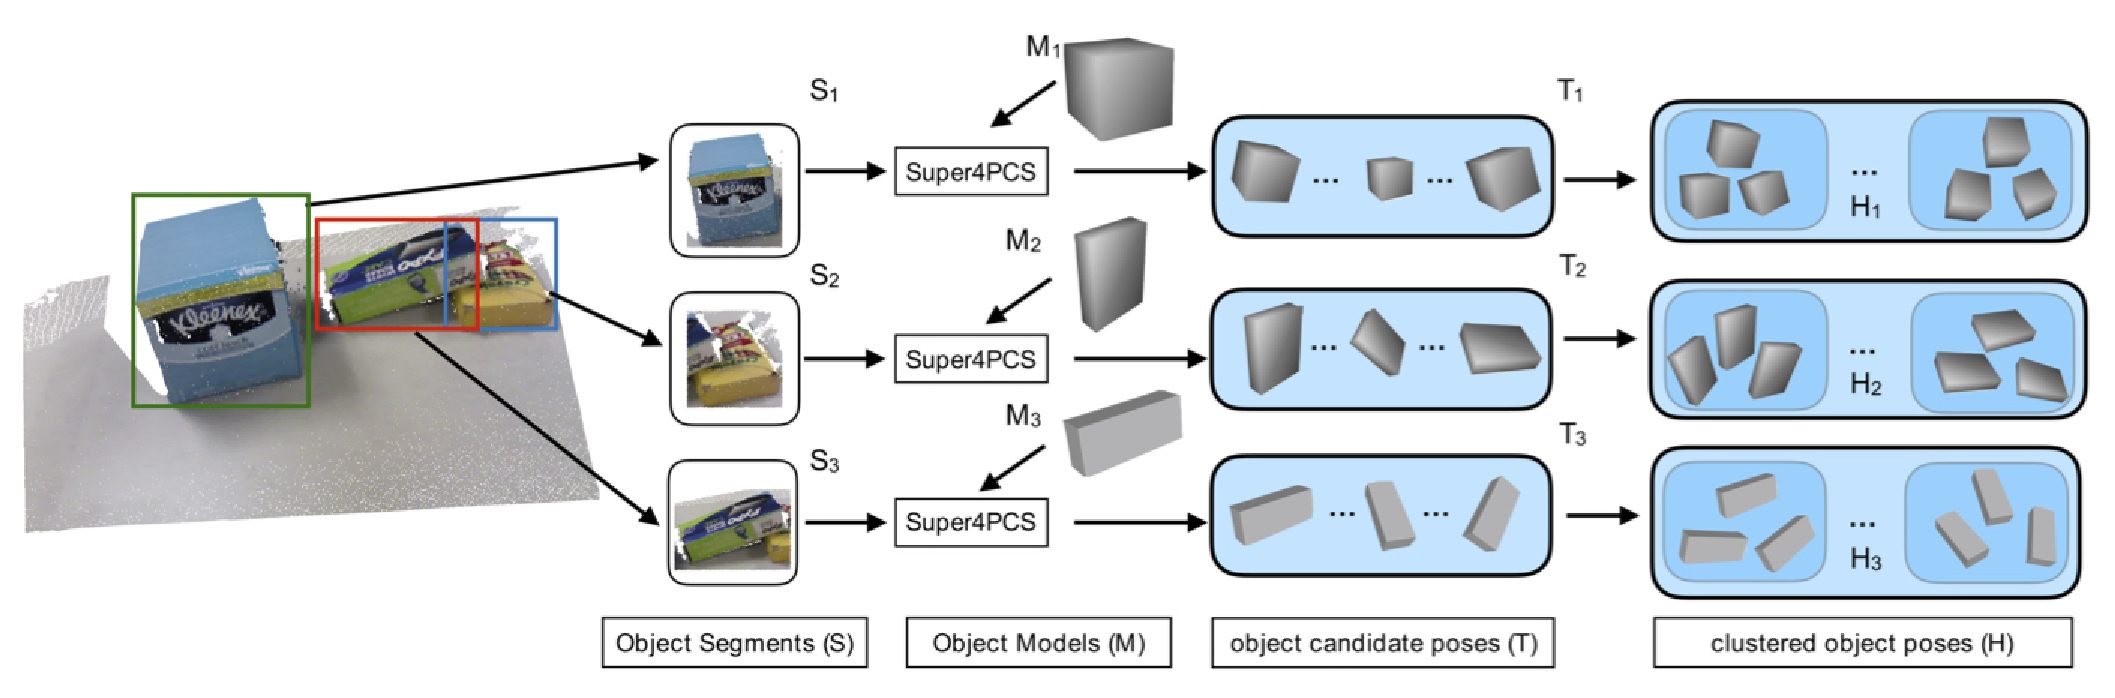
\includegraphics[width=0.9\textwidth]{clustering}
				\caption{object candidate pose generation and clustering to reduce set cardiniality}
			\end{figure}
			\vspace{-0.3in}
			\begin{itemize}
				\item Pose candidate set is constructed for each object using the extracted object segment and the 3D CAD model.
				\item For computational efficiency, the set of object hypotheses is clustered to obtain smaller candidate sets while still containing poses close to the true solutions. 
			\end{itemize}
			\vspace{-0.3in}
			\begin{columns}[t]
			\begin{column} {0.40\textwidth}
			\begin{figure}[h]
				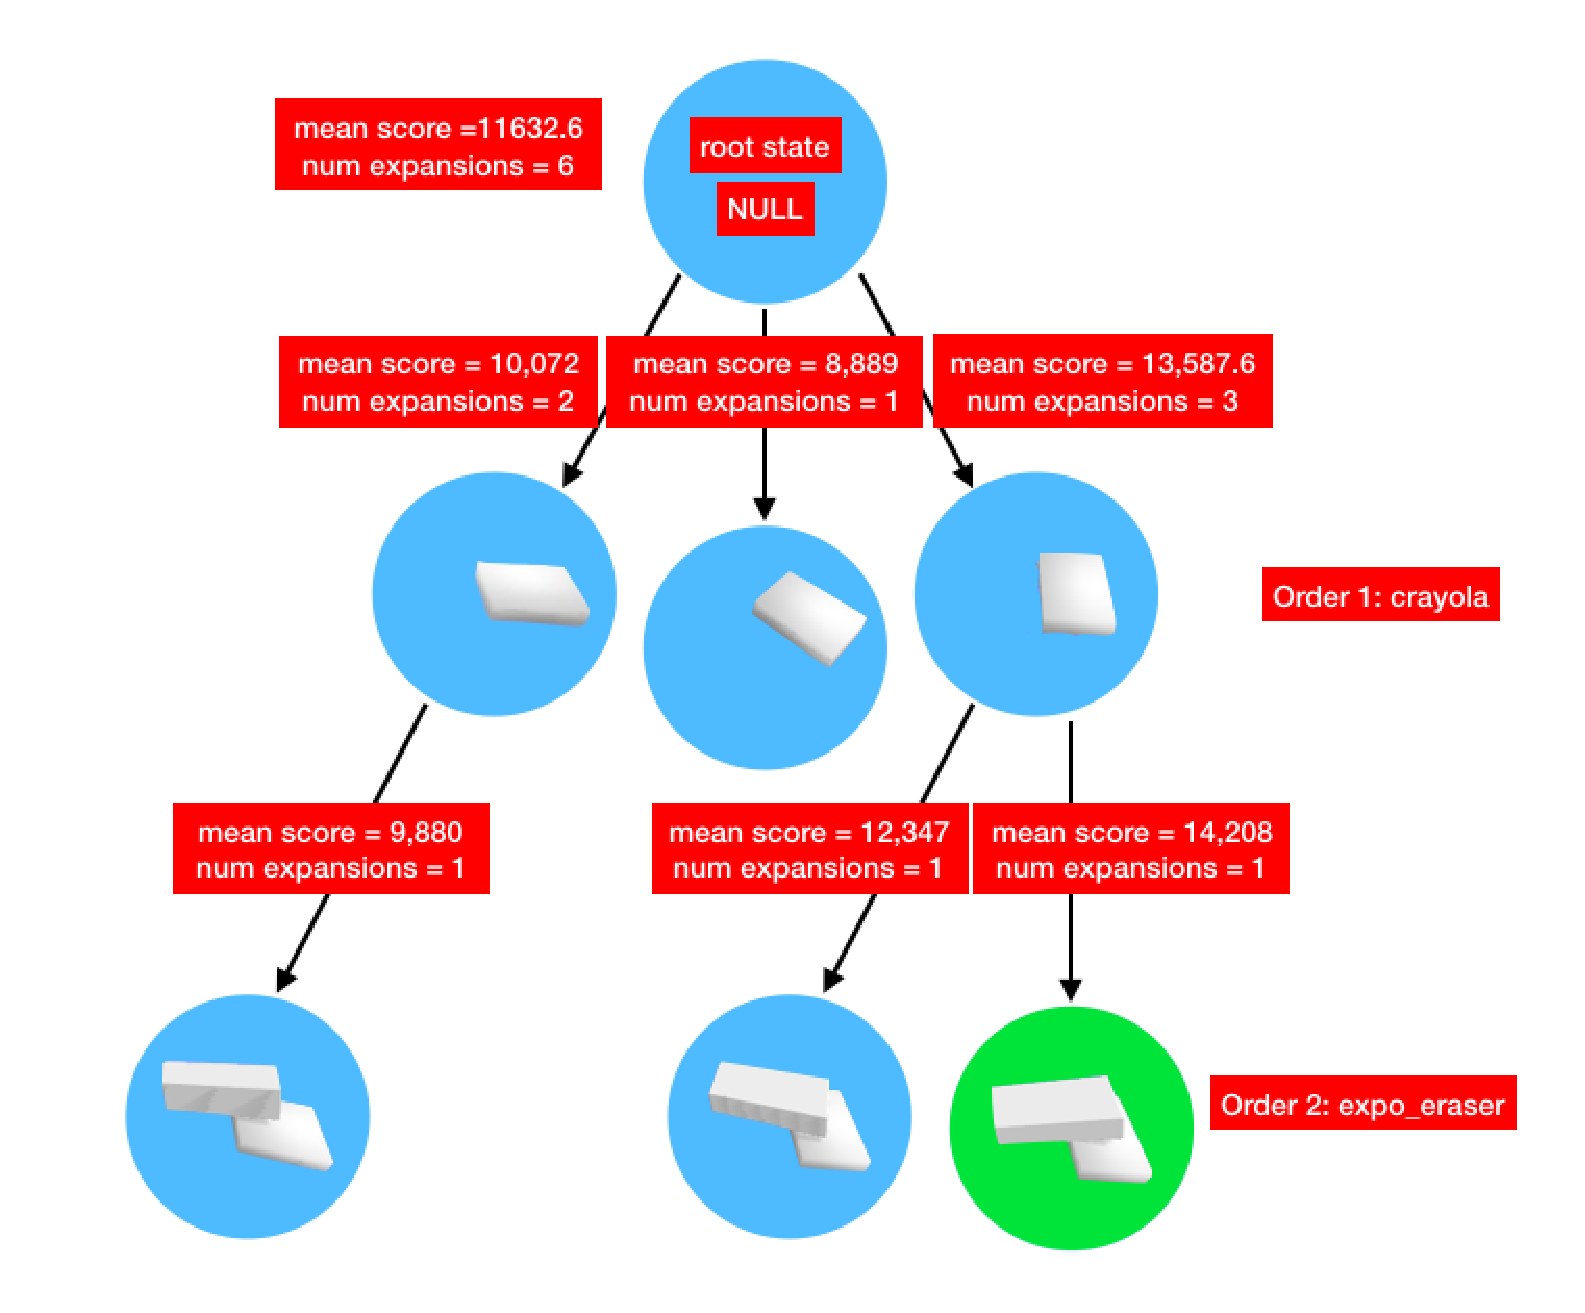
\includegraphics[width=0.8\textwidth]{mcts}
				\caption{Monte Carlo Tree Search for pose estimation}
			\end{figure}
			\end{column}
			\begin{column} {0.60\textwidth}
			\begin{itemize}
				\item An order of object placement is computed based on a set of rules defined over the object segments.
				\item Node expansion in the tree corresponds to an object placement, which is constrained (imposed by using physics simulator and point cloud trimming) by the previously placed objects.
				\item The leaf nodes (complete assignment) are rendered and a score is computed by comparing rendered scene to the observed depth image.
				\item The search uses Upper Confidence Bound to trade-off exploration and exploitation within the search.
			\end{itemize}
			\end{column}
			\end{columns}
		\end{block}
	\end{column}
	\begin{column}{0.30\textwidth}
		\begin{block}{\large Pose Estimation Evaluation}
			\centering
			\begin{itemize}
				\item Results demonstrate that search is useful in case of a clutter.
				\item MCTS converges much faster compared to using a heuristic based on registration score.
			\end{itemize}
			\vspace{-0.2in}
			\begin{figure}[h]
				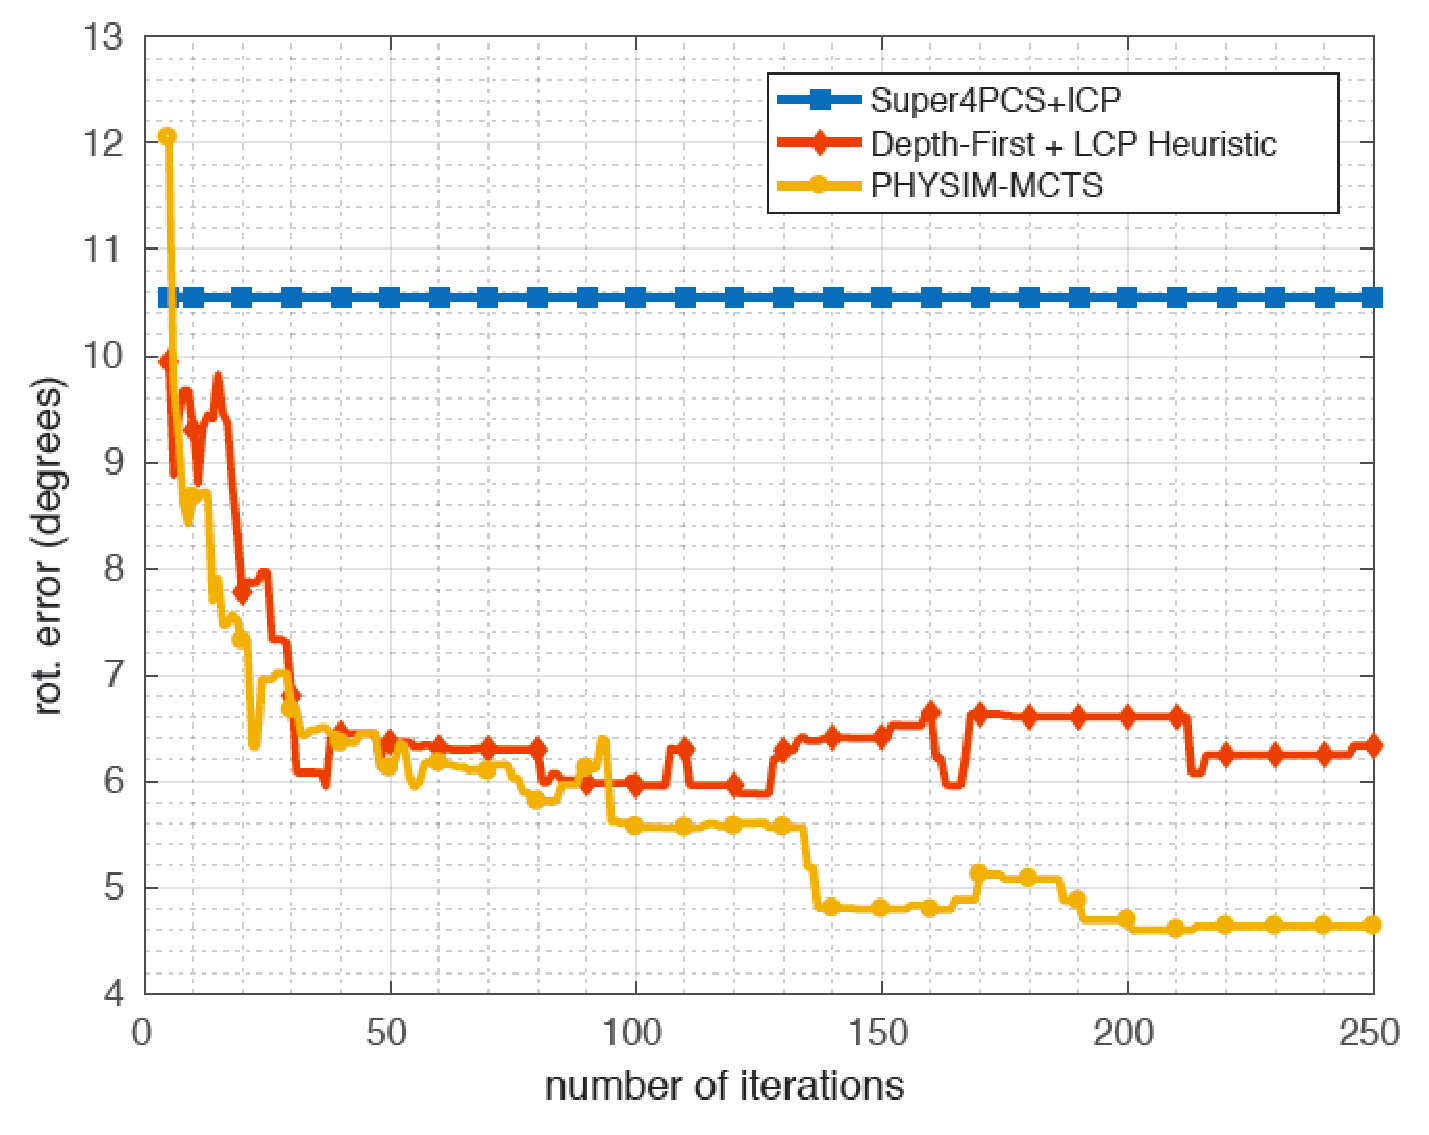
\includegraphics[width=0.75\textwidth]{graph1}
				\caption{Rotation error (degrees) vs the number of search expansions}
			\end{figure}
			\begin{figure}[h]
				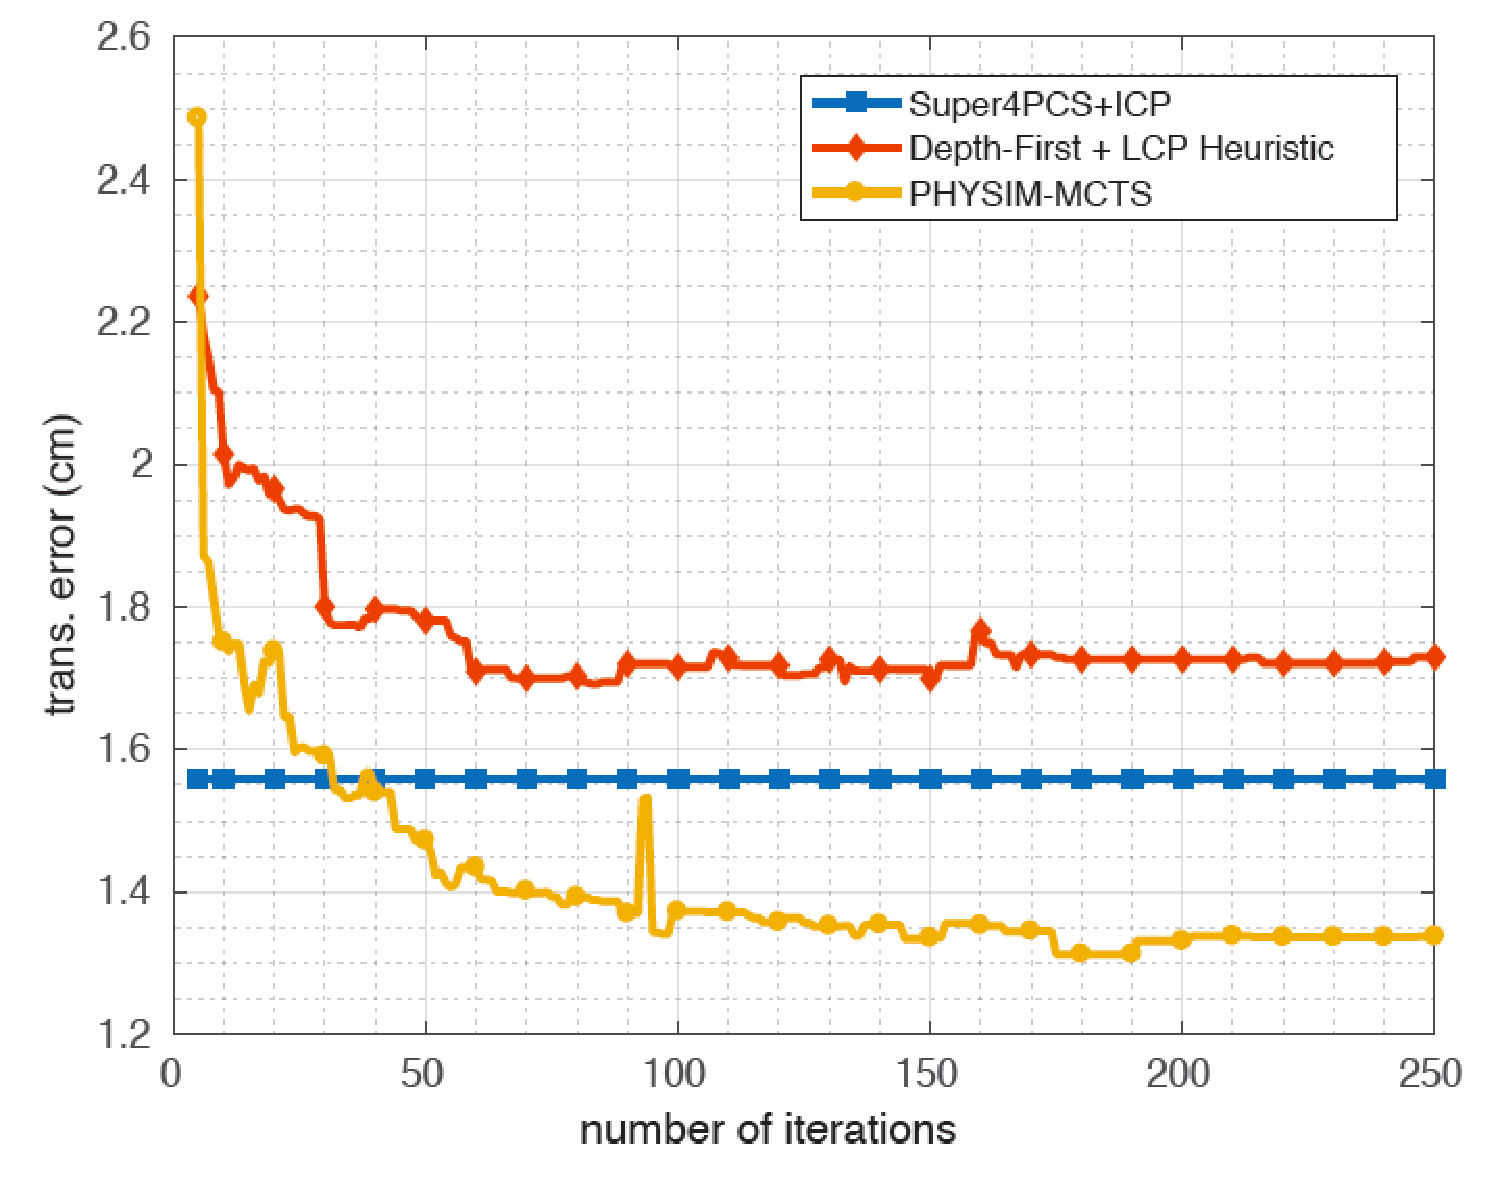
\includegraphics[width=0.75\textwidth]{graph2}
				\caption{Translational error (cms) vs the number of search expansions}
			\end{figure}
		\end{block}
	\end{column}
\end{columns}
    \vfill
  \end{frame}
\end{document}


%%%%%%%%%%%%%%%%%%%%%%%%%%%%%%%%%%%%%%%%%%%%%%%%%%%%%%%%%%%%%%%%%%%%%%%%%%%%%%%%%%%%%%%%%%%%%%%%%%%%
%%% Local Variables: 
%%% mode: latex
%%% TeX-PDF-mode: t
%%% End:
